% Informe en formato IEEE (conferencia, dos columnas).
% Compilar desde esta carpeta:  pdflatex informe.tex && pdflatex informe.tex
% IEEEtran.cls está incluido al lado para no depender de la instalación de TeX.

\documentclass[conference,a4paper]{IEEEtran}

\usepackage[utf8]{inputenc}
\usepackage[T1]{fontenc}
\usepackage{mathptmx}
\usepackage{amsmath,amssymb}
\usepackage{cite}
\usepackage{graphicx}
\usepackage{booktabs}
\usepackage{array}
\usepackage{xcolor}
\usepackage{listings}
\usepackage{tikz}
\usetikzlibrary{positioning,arrows.meta,fit,calc}
\usepackage[hidelinks]{hyperref}

% IEEEtran trae los rótulos en inglés y no hay babel-spanish instalado.
\renewcommand{\abstractname}{Resumen}
\renewcommand{\IEEEkeywordsname}{Palabras clave}
\renewcommand{\tablename}{TABLA}
\renewcommand{\refname}{Referencias}
\renewcommand{\lstlistingname}{Listado}

\lstset{
  basicstyle=\ttfamily\footnotesize,
  keywordstyle=\bfseries,
  columns=fullflexible,
  keepspaces=true,
  frame=tb,
  framesep=3pt,
  xleftmargin=2pt,
  literate={á}{{\'a}}1 {é}{{\'e}}1 {í}{{\'i}}1 {ó}{{\'o}}1 {ú}{{\'u}}1 {ñ}{{\~n}}1
}

% Sin patrones de español: se cortan a mano las palabras largas más frecuentes.
\hyphenation{par-ti-cio-nes pro-ce-sa-mien-to dis-tri-bui-do dis-tri-bui-dos
  i-te-ra-cio-nes cen-troi-de cen-troi-des e-je-cu-tor e-je-cu-to-res
  a-gru-pa-mien-to me-mo-ria trans-for-ma-cio-nes es-pe-cu-la-ti-va
  a-pli-ca-cio-nes al-go-rit-mo al-go-rit-mos ac-ti-vi-dad pro-yec-tor
  ce-lu-lar ce-lu-la-res es-tu-dian-tes per-sis-ten-cia bi-blio-te-ca
  a-pren-di-za-je}

\begin{document}

\title{Procesamiento distribuido y \textit{machine learning}\\sobre datos masivos con Apache Spark MLlib:\\K-Means distribuido como actividad en el aula}

\author{\IEEEauthorblockN{[Nombre y apellido]}
\IEEEauthorblockA{[Carrera] --- [Universidad]\\
Cátedra de Bases de Datos\\
{[correo institucional]}}}

\maketitle

\begin{abstract}
Cuando un conjunto de datos supera la capacidad de una sola computadora, su análisis exige repartir datos y cómputo entre muchas máquinas. Este informe presenta los fundamentos del procesamiento distribuido, desde el modelo MapReduce de Hadoop hasta Apache Spark y su abstracción de conjuntos de datos distribuidos resilientes (RDD), y describe cómo la biblioteca MLlib ejecuta el algoritmo K-Means sobre un clúster. Se analizan tres decisiones de diseño que explican el rendimiento y la robustez de Spark: la agregación de estadísticos suficientes (sumas y conteos) en lugar de promedios parciales, la persistencia en memoria entre iteraciones y la recuperación ante fallos por linaje. Por último, se describe una actividad web en tiempo real en la que el proyector del aula actúa como \textit{driver} y cada celular de los estudiantes como \textit{executor}, y se reportan los resultados de un ensayo con 24 nodos simulados.
\end{abstract}

\begin{IEEEkeywords}
Apache Spark, MLlib, MapReduce, Hadoop, K-Means, procesamiento distribuido, RDD, tolerancia a fallos, big data.
\end{IEEEkeywords}

\section{Introducción}

El volumen de datos que generan hoy las organizaciones (registros de transacciones, eventos de aplicaciones, sensores) crece más rápido que la capacidad de una única máquina para almacenarlos y procesarlos. Ante este límite hay dos caminos: escalar verticalmente, comprando una computadora más potente, o escalar horizontalmente, repartiendo el trabajo entre muchas computadoras comunes conectadas en red. El segundo camino es más barato y casi no tiene techo, pero introduce problemas nuevos: cómo dividir los datos, cómo coordinar las máquinas, cuánto tráfico de red se genera y qué hacer cuando una de ellas falla o se vuelve lenta.

Google formalizó una respuesta a estos problemas con el modelo MapReduce~\cite{dean2004mapreduce}, que Hadoop popularizó como software libre junto con su sistema de archivos distribuido HDFS~\cite{shvachko2010hdfs}. MapReduce resultó muy eficaz para trabajos de una sola pasada, pero ineficiente para los algoritmos iterativos típicos del aprendizaje automático, que recorren los mismos datos decenas de veces. Apache Spark~\cite{zaharia2010spark,zaharia2012rdd} nació precisamente para cubrir ese caso, manteniendo los datos en memoria entre iteraciones sin renunciar a la tolerancia a fallos.

Este trabajo tiene dos objetivos. El primero es explicar los conceptos centrales de Spark y de su biblioteca de aprendizaje automático, MLlib~\cite{meng2016mllib}, tomando como caso de estudio el algoritmo de agrupamiento K-Means. El segundo es presentar una actividad interactiva que permite a una clase vivir esos conceptos: cada estudiante se convierte en un nodo del clúster y procesa, desde su celular, una porción de los datos.

El resto del informe se organiza así: la Sección~\ref{sec:marco} presenta el marco teórico; la Sección~\ref{sec:kmeans} analiza K-Means y su paralelización; la Sección~\ref{sec:fallos} trata la tolerancia a fallos y el rendimiento; la Sección~\ref{sec:actividad} describe la actividad y sus resultados, y la Sección~\ref{sec:conclusiones} presenta las conclusiones.

\section{Marco teórico}
\label{sec:marco}

\subsection{El modelo MapReduce}

MapReduce~\cite{dean2004mapreduce} expresa un cómputo como dos funciones que escribe el programador. La función \textit{map} se aplica en paralelo a cada fragmento de la entrada y emite pares clave--valor; la función \textit{reduce} recibe todos los valores asociados a una misma clave y los combina. Entre ambas etapas, el sistema agrupa los pares por clave y los transfiere por la red (\textit{shuffle}). Opcionalmente, una función \textit{combiner} realiza una reducción parcial en cada nodo antes del \textit{shuffle}, lo que reduce el volumen transmitido cuando la operación es asociativa y conmutativa.

El sistema se encarga del resto: divide la entrada, asigna tareas a las máquinas, reintenta las que fallan y lanza copias de respaldo de las tareas más lentas. Para garantizar la tolerancia a fallos, cada trabajo lee su entrada desde el sistema de archivos distribuido y escribe allí su salida, replicada en varios discos. Esta decisión es simple y robusta, pero tiene un costo: un algoritmo iterativo debe encadenar un trabajo por iteración y paga en cada uno la lectura y la escritura completas en disco.

\subsection{Apache Spark y los RDD}

Spark~\cite{zaharia2010spark} se apoya en una abstracción llamada \textit{Resilient Distributed Dataset} (RDD)~\cite{zaharia2012rdd}: una colección inmutable de registros, dividida en particiones repartidas entre las máquinas del clúster. Sobre un RDD se definen dos clases de operaciones:

\begin{itemize}
\item \textbf{Transformaciones} (\texttt{map}, \texttt{filter}, \texttt{reduceByKey}, \ldots), que describen un RDD nuevo a partir de otro. Son \textit{perezosas}: no se ejecutan al declararse, sino que se registran en un grafo dirigido acíclico (DAG) de dependencias.
\item \textbf{Acciones} (\texttt{count}, \texttt{collect}, \texttt{save}, \ldots), que obligan a calcular un resultado y disparan la ejecución del DAG.
\end{itemize}

La evaluación perezosa permite al planificador ver el cómputo completo antes de ejecutarlo y fusionar en una misma etapa (\textit{stage}) las transformaciones con dependencias estrechas, es decir, aquellas en las que cada partición de salida depende de una sola partición de entrada. Las dependencias amplias, como un \texttt{reduceByKey}, requieren un \textit{shuffle} y marcan el límite entre etapas.

Dos propiedades distinguen a los RDD. La primera es la \textbf{persistencia}: el programador puede pedir con \texttt{cache()} o \texttt{persist()} que un RDD quede en la memoria de los nodos tras calcularse por primera vez, para reutilizarlo sin volver a leerlo del disco. La segunda es el \textbf{linaje} (\textit{lineage}): en lugar de replicar los datos intermedios, cada RDD recuerda qué transformaciones lo produjeron a partir de datos estables. Si se pierde una partición, Spark la recalcula aplicando de nuevo esa receta solamente sobre la porción afectada~\cite{zaharia2012rdd}.

En la versión actual, la mayoría de los programas usan la API de \textit{DataFrames} y Spark SQL, que agregan un esquema tabular y un optimizador de consultas sobre el mismo motor~\cite{zaharia2016unified}. Los conceptos de partición, DAG, persistencia y linaje se mantienen.

\subsection{Arquitectura de ejecución}

Una aplicación Spark se compone de los siguientes roles~\cite{spark-cluster}, ilustrados en la Fig.~\ref{fig:arquitectura}:

\begin{itemize}
\item \textbf{Driver}: el proceso que ejecuta el programa principal. Construye el DAG, lo divide en etapas y tareas, envía las tareas a los \textit{executors} y reúne los resultados.
\item \textbf{Cluster manager} (o \textit{master}): administra los recursos del clúster y asigna máquinas a cada aplicación. Puede ser el gestor \textit{standalone} de Spark, YARN~\cite{vavilapalli2013yarn} o Kubernetes. No procesa datos.
\item \textbf{Worker node}: cada máquina del clúster capaz de alojar procesos de la aplicación.
\item \textbf{Executor}: proceso que corre en un \textit{worker}, ejecuta tareas sobre particiones y conserva en su memoria los datos persistidos.
\end{itemize}

Una vez asignados los recursos, el \textit{driver} se comunica directamente con los \textit{executors}; el \textit{cluster manager} no interviene en el procesamiento.

\begin{figure}[t]
\centering
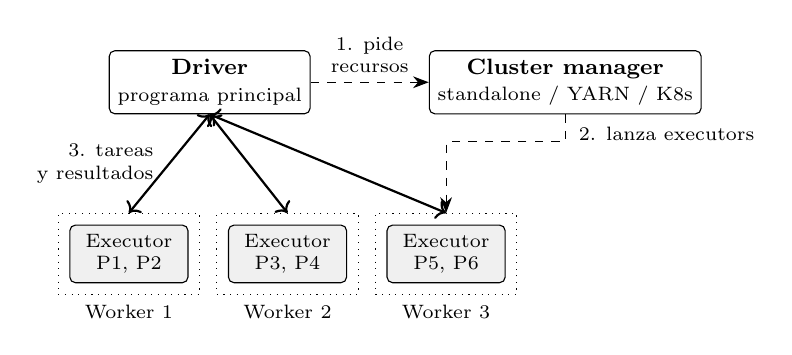
\begin{tikzpicture}[
  font=\footnotesize,
  box/.style={draw, rounded corners=2pt, minimum height=0.8cm, align=center, inner sep=3pt},
  exe/.style={draw, rounded corners=2pt, fill=black!6, minimum width=1.5cm, minimum height=0.55cm, align=center, font=\scriptsize},
  arr/.style={-{Stealth[length=2mm]}, thick},
  ctl/.style={-{Stealth[length=2mm]}, dashed}
]
\node[box, minimum width=2.3cm] (driver) {\textbf{Driver}\\\scriptsize programa principal};
\node[box, minimum width=2.3cm, right=1.5cm of driver] (cm) {\textbf{Cluster manager}\\\scriptsize standalone / YARN / K8s};

\node[exe, below=1.4cm of driver.south west, anchor=north west, xshift=-0.5cm] (e1) {Executor\\P1, P2};
\node[exe, right=0.5cm of e1] (e2) {Executor\\P3, P4};
\node[exe, right=0.5cm of e2] (e3) {Executor\\P5, P6};

\node[draw, dotted, fit=(e1), inner sep=4pt, label={[font=\scriptsize]below:Worker 1}] (w1) {};
\node[draw, dotted, fit=(e2), inner sep=4pt, label={[font=\scriptsize]below:Worker 2}] (w2) {};
\node[draw, dotted, fit=(e3), inner sep=4pt, label={[font=\scriptsize]below:Worker 3}] (w3) {};

\draw[ctl] (driver) -- node[above, font=\scriptsize, align=center] {1. pide\\recursos} (cm);
\draw[ctl] (cm.south) |- ++(0,-0.35) -| (w3.north);
\draw[arr, <->] (driver.south) -- (w2.north);
\draw[arr, <->] (driver.south) -- node[left, font=\scriptsize, align=right, xshift=-2pt] {3. tareas\\y resultados} (w1.north);
\draw[arr, <->] (driver.south) -- (w3.north);
\node[font=\scriptsize, anchor=west] at ($(cm.south)+(0.05,-0.25)$) {2. lanza executors};
\end{tikzpicture}
\caption{Arquitectura de una aplicación Spark. Las líneas punteadas son tráfico de control; las continuas, el intercambio de tareas y resultados. Cada executor procesa sus particiones (P1--P6).}
\label{fig:arquitectura}
\end{figure}

\subsection{MLlib}

MLlib es la biblioteca de aprendizaje automático de Spark~\cite{meng2016mllib}. Ofrece algoritmos de clasificación, regresión, agrupamiento, filtrado colaborativo y reducción de dimensionalidad, junto con herramientas para construir \textit{pipelines} de preparación de datos. Su principal ventaja es que el mismo programa que se prueba sobre una muestra en una notebook se ejecuta sin cambios sobre miles de millones de registros en un clúster.

\section{K-Means distribuido}
\label{sec:kmeans}

\subsection{El algoritmo}

Dado un conjunto de $n$ puntos $x_1,\ldots,x_n \in \mathbb{R}^d$ y un número $k$ de grupos, K-Means busca $k$ centroides $\mu_1,\ldots,\mu_k$ que minimicen la suma de los cuadrados de las distancias de cada punto a su centroide más cercano (WSSSE, \textit{within-set sum of squared errors}):
\begin{equation}
J = \sum_{i=1}^{n} \min_{j} \lVert x_i - \mu_j \rVert^2 .
\label{eq:costo}
\end{equation}

El algoritmo de Lloyd~\cite{lloyd1982,macqueen1967} aproxima una solución alternando dos pasos hasta que los centroides dejan de moverse:
\begin{enumerate}
\item \textbf{Asignación}: cada punto se asigna al centroide más cercano, $c(i) = \arg\min_j \lVert x_i - \mu_j \rVert^2$.
\item \textbf{Actualización}: cada centroide pasa a ser el promedio de los puntos que tiene asignados.
\end{enumerate}
Cada iteración no aumenta el costo $J$, por lo que el algoritmo converge, aunque puede hacerlo a un mínimo local que depende de los centroides iniciales.

\subsection{Paralelización con estadísticos suficientes}

El paso de asignación es trivialmente paralelo: cada \textit{executor} solo necesita sus puntos y los $k$ centroides actuales, que el \textit{driver} le envía. El paso de actualización, en cambio, requiere combinar información de todas las particiones. Para ello, cada \textit{executor} $p$ calcula, por cada grupo $j$, la suma de las coordenadas y la cantidad de puntos asignados:
\begin{equation}
S_{p,j} = \sum_{i \in p,\; c(i)=j} x_i, \qquad N_{p,j} = \bigl|\{ i \in p : c(i)=j \}\bigr| .
\end{equation}
El \textit{driver} suma estos valores y divide una sola vez:
\begin{equation}
\mu_j' = \frac{\sum_p S_{p,j}}{\sum_p N_{p,j}} .
\label{eq:centroide}
\end{equation}

El par $(S, N)$ es un estadístico suficiente: contiene toda la información necesaria para calcular el promedio global y su combinación es asociativa y conmutativa, por lo que puede reducirse en árbol o en cualquier orden. El tamaño del mensaje es $k(d+1)$ números por partición, independiente de la cantidad de puntos. MLlib implementa así cada iteración: una agregación de sumas y conteos por grupo sobre el RDD persistido~\cite{meng2016mllib}.

\subsection{El error del promedio de promedios}

Una alternativa tentadora es que cada \textit{executor} envíe directamente el promedio de sus puntos por grupo, $\bar{x}_{p,j} = S_{p,j}/N_{p,j}$, y que el \textit{driver} promedie esos promedios. El resultado es incorrecto siempre que las particiones tengan distinta cantidad de puntos en un mismo grupo, porque se pierde el peso $N_{p,j}$. Por ejemplo, si una partición tiene un único punto en $x=10$ y otra tiene tres puntos en $x=0$:
\begin{equation}
\underbrace{\frac{10 + 0}{2} = 5}_{\text{promedio de promedios}}
\quad\neq\quad
\underbrace{\frac{10 + 0 + 0 + 0}{4} = 2{,}5}_{\text{promedio real}} .
\end{equation}

La Tabla~\ref{tab:mensajes} compara las tres estrategias que la actividad propone a los estudiantes, con $k=3$, $d=2$ y valores de 8 bytes.

\begin{table}[t]
\caption{Qué envía cada executor al driver en una iteración}
\label{tab:mensajes}
\centering
\begin{tabular}{@{}l>{\raggedright\arraybackslash}p{2.2cm}cc@{}}
\toprule
\textbf{Opción} & \textbf{Contenido} & \textbf{Tamaño} & \textbf{Correcto} \\
\midrule
A & Todos los puntos & $\propto n$ (19~MiB para $10^6$) & Sí \\
B & Promedio por grupo & 48~B & No \\
C & Suma y conteo por grupo & 72~B & Sí \\
\bottomrule
\end{tabular}
\end{table}

La opción~A es correcta pero traslada todos los datos al \textit{driver}, lo que anula la ventaja de distribuir y convierte al \textit{driver} en un cuello de botella. La opción~B es pequeña pero incorrecta. La opción~C es pequeña y correcta: es el patrón de \textit{combiner} de MapReduce aplicado a K-Means.

\subsection{Inicialización y parámetros en MLlib}

Como el resultado depende de los centroides iniciales, MLlib usa por defecto la inicialización \textit{k-means$\|$}~\cite{bahmani2012scalable}, una variante paralelizable de \textit{k-means++} que elige centroides iniciales dispersos en pocas pasadas sobre los datos. Los parámetros principales del estimador \texttt{pyspark.ml.clustering.KMeans} son la cantidad de grupos \texttt{k}, el máximo de iteraciones \texttt{maxIter} (20 por defecto), la tolerancia de convergencia \texttt{tol} y la semilla \texttt{seed}~\cite{spark-mllib}. El Listado~\ref{lst:pyspark} muestra un programa completo.

\begin{lstlisting}[language=Python, caption={K-Means con PySpark y MLlib}, label={lst:pyspark}]
from pyspark.ml.clustering import KMeans
from pyspark.ml.feature import VectorAssembler

df = spark.read.csv("clientes.csv",
                    header=True, inferSchema=True)
vec = VectorAssembler(inputCols=["x", "y"],
                      outputCol="features")
datos = vec.transform(df).cache()

modelo = KMeans(k=3, maxIter=12, seed=1).fit(datos)
print(modelo.clusterCenters())
print(modelo.summary.trainingCost)  # WSSSE
\end{lstlisting}

La llamada a \texttt{cache()} es la que convierte a Spark en una herramienta adecuada para este algoritmo: sin ella, cada iteración volvería a leer y a convertir el archivo de entrada.

\section{Tolerancia a fallos y rendimiento}
\label{sec:fallos}

\subsection{Recuperación por linaje}

En un clúster de cientos de máquinas, las fallas son eventos normales. MapReduce y HDFS las toleran replicando los datos en disco; Spark, en cambio, reconstruye las particiones perdidas a partir de su linaje~\cite{zaharia2012rdd}. Si un \textit{executor} se cae durante una iteración de K-Means, el \textit{driver} detecta que sus tareas no terminaron y las reasigna a otros \textit{executors}, que vuelven a leer la porción correspondiente de la entrada, reaplican las transformaciones y continúan. Solo se recalcula lo perdido, sin replicar en memoria cada resultado intermedio.

\subsection{Rezagados y ejecución especulativa}

Como cada iteración termina cuando termina su tarea más lenta, una sola máquina rezagada (\textit{straggler}), por un disco degradado o por competir con otros procesos, retrasa a todo el clúster. Dean y Ghemawat propusieron lanzar \textit{tareas de respaldo}: cuando el trabajo está por terminar, las tareas que siguen en curso se copian en otras máquinas y se usa el resultado de la que termine primero~\cite{dean2004mapreduce}. Spark implementa la misma idea con la opción \texttt{spark.speculation}, desactivada por defecto. Al activarla, una tarea se relanza cuando dura más que un múltiplo (\texttt{spark.speculation.multiplier}, 3 en la documentación actual) de la mediana de las tareas de su etapa, una vez completada una fracción de ellas (\texttt{spark.speculation.quantile}, 0,9)~\cite{spark-config}.

\subsection{Spark frente a Hadoop en algoritmos iterativos}

Sea $r$ el tiempo de leer una partición desde el disco, $c$ el de procesarla y $w$ el de escribir el resultado intermedio. Para $m$ iteraciones, un encadenamiento de trabajos MapReduce cuesta aproximadamente
\begin{equation}
T_{\text{Hadoop}} \approx m\,(r + c + w),
\end{equation}
mientras que Spark, con los datos persistidos en memoria, lee una sola vez:
\begin{equation}
T_{\text{Spark}} \approx r + m\,c .
\end{equation}
Cuando la lectura domina ($r \gg c$), la ventaja crece casi linealmente con la cantidad de iteraciones. Zaharia et al. reportaron mejoras de hasta 20 veces en algoritmos iterativos de aprendizaje automático~\cite{zaharia2012rdd}. La Tabla~\ref{tab:comparacion} resume las diferencias.

\begin{table}[t]
\caption{Hadoop MapReduce y Apache Spark}
\label{tab:comparacion}
\centering
\begin{tabular}{@{}>{\raggedright\arraybackslash}p{1.9cm}>{\raggedright\arraybackslash}p{2.6cm}>{\raggedright\arraybackslash}p{2.6cm}@{}}
\toprule
& \textbf{Hadoop MapReduce} & \textbf{Spark} \\
\midrule
Datos entre pasos & Disco (HDFS) & Memoria (\texttt{cache}) \\
Modelo & Map y reduce fijos & DAG de transformaciones \\
Tolerancia a fallos & Replicación en disco & Linaje y recálculo \\
Iterativo & Un trabajo por iteración & Un programa, datos reutilizados \\
APIs & Java & Scala, Java, Python, R, SQL \\
\bottomrule
\end{tabular}
\end{table}

Spark no es siempre la mejor opción. Si los datos caben en la memoria de una sola máquina, bibliotecas locales como pandas o scikit-learn suelen ser más rápidas, porque evitan el costo de coordinar procesos, serializar datos y transmitirlos por la red. El procesamiento distribuido se justifica cuando el volumen o el tiempo de cómputo superan lo que una máquina puede resolver.

\section{Actividad propuesta: ``Sos un nodo''}
\label{sec:actividad}

\subsection{Objetivo y diseño}

Para que los conceptos anteriores se comprendan por experiencia y no solo por exposición, se diseñó una actividad web de unos 15 minutos para un curso de alrededor de 30 estudiantes. El proyector del aula muestra la consola del \textit{driver} y cada estudiante se une escaneando un código QR: su celular pasa a ser un \textit{executor} que recibe una partición de 8 puntos de un conjunto de datos sintético de clientes con tres segmentos ocultos.

El sistema está implementado en Node.js con Express y Socket.io. Un servidor central mantiene el estado autoritativo de la simulación (particiones, centroides, tareas en curso) y lo sincroniza con el proyector y con los celulares mediante WebSockets. Puede servirse desde una computadora personal y publicarse a través de un túnel de Cloudflare, sin servicios de terceros para almacenar datos. Un modo de alto contraste permite usarlo con el aula iluminada.

\subsection{Fases}

La Tabla~\ref{tab:fases} resume las fases y el concepto que ilustra cada una.

\begin{table}[t]
\caption{Fases de la actividad}
\label{tab:fases}
\centering
\begin{tabular}{@{}>{\raggedright\arraybackslash}p{1.6cm}>{\raggedright\arraybackslash}p{3.3cm}>{\raggedright\arraybackslash}p{2.3cm}@{}}
\toprule
\textbf{Fase} & \textbf{Qué hacen los estudiantes} & \textbf{Concepto} \\
\midrule
Unirse & Escanean el QR y reciben su partición & Driver, executor, partición \\
Map a mano & Asignan sus puntos al centroide más cercano y eligen qué enviar (A, B o C) & Paso map, costo de red \\
Reduce & Observan el error que introduce B y el volumen de A & Combiner, estadísticos suficientes \\
Modo Spark & Sus celulares calculan solos varias iteraciones; un nodo se vuelve lento & Iteración, rezagados, ejecución especulativa \\
Fallos & Se ``matan'' nodos en vivo & Linaje y recálculo \\
Hadoop vs.\ Spark & Corre el mismo trabajo con y sin \texttt{cache()} & Persistencia en memoria \\
Código & Ven el programa PySpark con los valores de su corrida & MLlib \\
\bottomrule
\end{tabular}
\end{table}

\subsection{Ensayo y resultados}

La actividad se ensayó con 24 \textit{executors} simulados por un programa auxiliar y un celular real. En la fase manual, los nodos que eligieron la opción~B desplazaron visiblemente un centroide respecto del valor correcto, que el proyector muestra como un centroide ``fantasma''. En el modo Spark, el algoritmo convergió en dos iteraciones partiendo de los centroides calculados a mano. Al marcar un nodo como lento, la copia especulativa lanzada en un nodo libre terminó antes que la original, y al desconectar nodos sus particiones se reasignaron a otros \textit{executors} sin reiniciar el trabajo.

En la carrera de 5 iteraciones, el modo Hadoop tardó 23,3~s y el modo Spark 9,5~s, una mejora de 2,4 veces. Estos tiempos no son una medición de Hadoop ni de Spark reales: surgen de latencias simuladas (1,1~s de lectura y 0,5~s de escritura por tarea en el modo Hadoop, frente a una única lectura en el modo Spark) más la comunicación con los dispositivos. Su propósito es didáctico: hacer visible, en la escala de tiempo de una clase, la diferencia que formaliza el modelo de costos anterior.

\subsection{Limitaciones}

La actividad simplifica deliberadamente varios aspectos. No representa al \textit{cluster manager}, porque los celulares ya están conectados al iniciar; cada celular cumple a la vez el papel de \textit{worker} y de \textit{executor}, y los datos son bidimensionales para poder dibujarlos. El servidor central es un punto único de falla, igual que el \textit{driver} en Spark: si se detiene, la actividad debe reiniciarse.

\section{Conclusiones}
\label{sec:conclusiones}

Apache Spark resuelve el principal límite de MapReduce para el aprendizaje automático, el costo de releer los datos en cada iteración, mediante la persistencia en memoria, y conserva la tolerancia a fallos gracias al linaje en lugar de la replicación. K-Means muestra con claridad estas ideas: su paso de asignación es paralelo por naturaleza y su paso de actualización se distribuye correctamente solo si los nodos envían estadísticos combinables, como sumas y conteos, y no resultados ya agregados, como promedios. La actividad propuesta traslada estos conceptos a una experiencia colectiva en la que cada estudiante procesa datos, comete o evita el error del promedio de promedios, sufre la caída de un nodo y compara el costo del disco con el de la memoria, antes de ver que MLlib resume todo ese trabajo en pocas líneas de código.

\begin{thebibliography}{99}

\bibitem{dean2004mapreduce}
J.~Dean and S.~Ghemawat, ``MapReduce: Simplified data processing on large clusters,'' in \textit{Proc. 6th USENIX Symp. Operating Systems Design and Implementation (OSDI)}, San Francisco, CA, USA, 2004, pp.~137--150.

\bibitem{shvachko2010hdfs}
K.~Shvachko, H.~Kuang, S.~Radia, and R.~Chansler, ``The Hadoop distributed file system,'' in \textit{Proc. IEEE 26th Symp. Mass Storage Systems and Technologies (MSST)}, 2010, pp.~1--10.

\bibitem{zaharia2010spark}
M.~Zaharia, M.~Chowdhury, M.~J. Franklin, S.~Shenker, and I.~Stoica, ``Spark: Cluster computing with working sets,'' in \textit{Proc. 2nd USENIX Workshop Hot Topics in Cloud Computing (HotCloud)}, 2010.

\bibitem{zaharia2012rdd}
M.~Zaharia \textit{et al.}, ``Resilient distributed datasets: A fault-tolerant abstraction for in-memory cluster computing,'' in \textit{Proc. 9th USENIX Symp. Networked Systems Design and Implementation (NSDI)}, San Jose, CA, USA, 2012, pp.~15--28.

\bibitem{zaharia2016unified}
M.~Zaharia \textit{et al.}, ``Apache Spark: A unified engine for big data processing,'' \textit{Commun. ACM}, vol.~59, no.~11, pp.~56--65, 2016.

\bibitem{meng2016mllib}
X.~Meng \textit{et al.}, ``MLlib: Machine learning in Apache Spark,'' \textit{J. Mach. Learn. Res.}, vol.~17, no.~34, pp.~1--7, 2016.

\bibitem{vavilapalli2013yarn}
V.~K. Vavilapalli \textit{et al.}, ``Apache Hadoop YARN: Yet another resource negotiator,'' in \textit{Proc. 4th ACM Symp. Cloud Computing (SoCC)}, 2013, pp.~5:1--5:16.

\bibitem{lloyd1982}
S.~Lloyd, ``Least squares quantization in PCM,'' \textit{IEEE Trans. Inf. Theory}, vol.~28, no.~2, pp.~129--137, 1982.

\bibitem{macqueen1967}
J.~MacQueen, ``Some methods for classification and analysis of multivariate observations,'' in \textit{Proc. 5th Berkeley Symp. Mathematical Statistics and Probability}, vol.~1, 1967, pp.~281--297.

\bibitem{bahmani2012scalable}
B.~Bahmani, B.~Moseley, A.~Vattani, R.~Kumar, and S.~Vassilvitskii, ``Scalable k-means++,'' \textit{Proc. VLDB Endowment}, vol.~5, no.~7, pp.~622--633, 2012.

\bibitem{spark-cluster}
The Apache Software Foundation, ``Cluster mode overview,'' \textit{Apache Spark Documentation}. [Online]. Available: \url{https://spark.apache.org/docs/latest/cluster-overview.html} (accedido: nov. 2026).

\bibitem{spark-mllib}
The Apache Software Foundation, ``Clustering --- K-means,'' \textit{Apache Spark MLlib Guide}. [Online]. Available: \url{https://spark.apache.org/docs/latest/ml-clustering.html} (accedido: nov. 2026).

\bibitem{spark-config}
The Apache Software Foundation, ``Spark configuration,'' \textit{Apache Spark Documentation}. [Online]. Available: \url{https://spark.apache.org/docs/latest/configuration.html} (accedido: nov. 2026).

\end{thebibliography}

\end{document}
